\documentclass[11pt]{article}

\usepackage[margin=1in]{geometry}
\usepackage{amsfonts, amsmath, amssymb}
\usepackage[none]{hyphenat}
\usepackage{fancyhdr}
\usepackage{graphicx}
\usepackage{float}
\usepackage[nottoc, notlot, notlof]{tocbibind}
\usepackage{hyperref}

\pagestyle{fancy}
\fancyhead{}
\fancyfoot{}
\fancyhead[L]{\slshape \MakeUppercase{Radio}}
\fancyhead[R]{\slshape Diagrams}
\fancyfoot[C]{\thepage}
\renewcommand{\footrulewidth}{0pt}

\parindent 0ex %
\renewcommand{\baselinestretch}{1.5}

\begin{document}

\begin{titlepage}
\begin{center}
\vspace*{1cm}
\Large{\textbf{Software Modeling}}\\
\Large{\textbf{Modeling and Implementation Phase}}
\vfill
\line(1,0){400}\\[1mm]
\huge{\textbf{“Radio Simulation”}}\\[3mm]
\Large{\textbf{- Diagrams -}}\\[1mm]
\line(1,0){400}\\
\vfill
By ESSAFSYFY Abdelkrim and MELUZOLA KIMFUTA Gingu\\
Academic year 2019-2020
\end{center}
\end{titlepage}

\tableofcontents
\thispagestyle{empty}
\clearpage
\setcounter{page}{1}

\section{Use case diagram}
\subsection{Diagram}
\vspace{10px}
\begin{center}
\includegraphics[width=15cm]{../Diagrams/useCase-v4.jpg}\\
\end{center}

\subsection{Diagram description}
The use case diagram for this project (radio simulation) has been made with the idea of two separate functionality categories:\\
Primary: the functionalitites that are present in each and every radio.\\
Secondary: the optional features that the manufacutrer (in this case the radio configurator\footnote{See Models' report}) chooses to add to the radio.
In the diagram, we notice these two categories in from of two abstract use cases named "Use primary dashboard" and "Use secondary dashboard". There are also four separate use cases; "Turn on/off" which will allow the user to manually turn the radio on and off, "Broadcast radio feed" by the radio stations, "Add/remove optional feature" and "Update existing features" by the radio constructor.\\
It is noteworthy that the use case "Use navigation controls" allows the user not only to choose what the radio's screen displays but also configure two use cases which are: "Change date and time" and "Activate/deactivate alarm", for the latter it is for the purpose of setting the time of the alarm, the activation/deactivation is done by another button.

\subsection{Individual use cases' description}
\subsubsection{Turn on/off}
\textbf{Use case name:} Turn on/off\\
\textbf{Summary:} Allows the user to turn the radio on or off.\\
\textbf{Actors:} User.\\
\textbf{Assumptions:} Radio has access to a power source.\\
\textbf{Preconditions:} Radio is plugged in.\\
\textbf{Basic course of action:}\\
\hspace*{10mm}1. User presses power button on.\\
\hspace*{10mm}2. LED indicator switches from red to green.\\
\hspace*{10mm}3. Radio is powered on.\\
\textbf{Postconditions: }The power button is functional.\\
\textbf{Alternate courses :}\\
\hspace*{10mm}1a. Alarm (if set) turns the radio on, on the programmed time.\\ 
\hspace*{10mm}3a. Radio is powered off.
\begin{center}--------\end{center}

\subsubsection{Use primary dashboard}
\textbf{Use case name}: Use primary dashboard\\
\textbf{Summary}: An abstract use case that allows the user to use the primary radio functionalities. Every specialization of this use case inherits its actors, assumptions, preconditions and postconditions.\\
\textbf{Actors}: User.\\
\textbf{Assumptions}: Radio is plugged in.\\
\textbf{Preconditions}: Radio is powered on.\\
\textbf{Basic course of action:}\\
\hspace*{10mm}1. User chooses to use one of the available functionalitites.
\begin{center}--------\end{center}

\subsubsection{Select radio station}
\textbf{Use case name}: Select radio station\\
\textbf{Summary}: Allows the user to select a radio station using a turn knob\\
\textbf{Actors}: User\\
\textbf{Assumptions}: Same as parent\\
\textbf{Preconditions}: Radio stations are available.\\
\textbf{Basic course of action:}\\
\hspace*{10mm}1. User turns knob until signal is good enough to produce sound\\
\hspace*{10mm}2. Radio plays radio station according to frequency\\
\hspace*{10mm}3. Radio automatically synchronization of date and time using the received signal\\
\textbf{Alternate courses: }\\
\hspace*{10mm}1a. User clicks one of the preset buttons\\
\hspace*{20mm}1a1. No station is saved into the pressed preset\\
\hspace*{20mm}1a2. Signal received is not good enough\\
\hspace*{20mm}1a3. Preset button is damaged, the radio doesn't play\\
\hspace*{10mm}2a. No radio station with good signal found\\
\hspace*{10mm}3a. The date and time are unsynchronized, the radio proceeds to automatically set the date and time.
\begin{center}--------\end{center}

\subsubsection{Turn volume up/down}
\textbf{Use case name}: Turn volume up/down\\
\textbf{Summary}: Allows the user to adjust the radio's volume from 0 to 20 in discrete steps.\\
\textbf{Actors}: User.\\
\textbf{Assumptions}  Same as parent.\\
\textbf{Preconditions}: Built-in speaker.\\
\textbf{Basic course of action:}\\
\hspace*{10mm}1. User turns the knob left or right to adjust the volume.\\
\hspace*{10mm}2. Radio changes the volume accordingly.\\
\textbf{Alternate courses:}\\
\hspace*{10mm}2a. The knob is damaged, the radio is unable to change the volume.
\begin{center}--------\end{center}

\subsubsection{Use navigation controls}
\textbf{Use case name}: Use navigation controls\\
\textbf{Summary:} Allows the user to change the display's content depending on its size.\\
\textbf{Actors:} User\\
\textbf{Assumptions:} Same as parent\\
\textbf{Preconditions:} Radio has a functioning screen\\
\textbf{Basic course of action:}\\
\hspace*{10mm}1. User uses navigation controls (Up, down, left, right) to choose was type of information is displayed on the screen. This includes displaying of date and time and alarm activation.\\
\hspace*{10mm}2. Radio changes the display's content accordingly\\
\textbf{Alternate courses:}\\
\hspace*{10mm}1a. The navigation controls are damaged, the user is unable to choose the type of information the screen displays.
\begin{center}--------\end{center}

\subsubsection{Change date and time}
\textbf{Use case name}: Change date and time\\
\textbf{Summary}: Allows the user to change the date and time of the radio\\
\textbf{Actors}: User\\
\textbf{Assumptions}: Same as parent\\
\textbf{Preconditions}: Radio is turned on\\
\textbf{Basic course of action:}\\
\hspace*{10mm}1. User changes date and time using navigation controls (see use case: navigation controls)
\textbf{Alternate courses: }\\
\hspace*{10mm}1a. Navigation controls are damaged, the user is unable to change the date and time.
\begin{center}--------\end{center}

\subsubsection{Save radio station to preset}
\textbf{Use case name:} Save radio station to preset\\
\textbf{Summary:} Allows the user to save the currently playing radio station to one of the free available presets (ranging from 3 to 10)\\
\textbf{Actors:} User\\
\textbf{Assumptions:} Same as parent\\
\textbf{Preconditions:} Radio station is playing\\
\textbf{Basic course of action:}\\
\hspace*{10mm}1. User holds the preset button during at least 3 seconds\\
\hspace*{10mm}2. Radio saves the currently playing station to the selected preset\\
\textbf{Alternate courses:}\\
\hspace*{10mm}1a. The selected preset already has a saved station\\
\hspace*{20mm}1a1. The radio overrides the old station with the new on\\
\hspace*{10mm}1b. The selected preset is damaged, the station cannot be saved\\
\hspace*{10mm}1c. No free presets are available, the user chooses not to override any
\begin{center}--------\end{center}

\subsubsection{Use secondary dashboard}
\textbf{Use case name}: Use secondary dashboard\\
\textbf{Summary}: An abstract use case that allows the user to use the secondary (optional) radio functionalities. Every specialization of this use case inherits its actors, assumptions, preconditions and postconditions.\\
\textbf{Actors}: User.\\
\textbf{Assumptions}: Radio is plugged in.\\
\textbf{Preconditions}: Radio is powered on.\\
\textbf{Basic course of action:}\\
\hspace*{10mm}1. User chooses to use one of the available functionalitites.
\begin{center}--------\end{center}

\subsubsection{Autotune radio station}
\textbf{Use case name:} Autotune radio station\\
\textbf{Summary:} Allows the user to use autotune functionality which will automatically search
for all available radio stations and will store them in its internal memory in the order they were found  until all memory locations are filled or until no more radio stations are found\\
\textbf{Actors:} User\\
\textbf{Assumptions:} Same as parent\\
\textbf{Preconditions:} Radio has autotune functionality\\
\textbf{Basic course of action:}\\
\hspace*{10mm}1. User activates autotune functionality using a button\\
\hspace*{10mm}2. Radio scans for all the stations available with good quality\\
\hspace*{10mm}3. Radio stores the fetched stations into its internal memory\\
\hspace*{10mm}4. User browses the stations found\\
\textbf{Alternate courses:}\\
\hspace*{10mm}1a. Autotune button is damaged, the functionality is unavailable\\
\hspace*{10mm}2a. No stations with good enough quality are found\\
\hspace*{10mm}2b. Radio's search functionality is damaged, it is unable to search for any station\\
\hspace*{10mm}3a. Radio's internal memory is damaged, no stations are stored\\
\hspace*{10mm}4a. User saves the playing station into a preset (see "Save radio station to preset" use case)\\
\hspace*{10mm}4b. User saves all found stations into all available presets.\\
\hspace*{20mm}4b1. Radio saves stations into presets until no more stations are found or no free presets remain.
\begin{center}--------\end{center}

\subsubsection{Adjust stereo balance}
\textbf{Use case name:} Use external audio output\\
\textbf{Summary:} Allows the user to adjust stereo balance by turning a knob which controls the output volume between the left and right speaker\\
\textbf{Actors:} User\\
\textbf{Assumptions:} Same as parent\\
\textbf{Preconditions:} Radio has two built-in speakers\\
\textbf{Basic course of action:}\\
\hspace*{10mm}1. User turns the knob left or right\\
\hspace*{10mm}2. Radio adjusts the stereo balance accordingly\\
\textbf{Alternate courses:}\\
\hspace*{10mm}2a. Stereo balance knob is damaged, no audio change will result
\begin{center}--------\end{center}

\subsubsection{Use external audio input}
\textbf{Use case name:} Use external audio input\\
\textbf{Summary:} Allows the user to plug in an external audio input allowing the radio to receive sound from an external device.\\
\textbf{Actors:} User\\
\textbf{Assumptions:} Same as parent\\
\textbf{Preconditions:} External audio input functionality available\\
\textbf{Basic course of action:}\\
\hspace*{10mm}1. User establishes connection (USB, audio jack or bluetooth) with the radio\\
\hspace*{10mm}2. Radio detects the external audio input\\
\hspace*{10mm}3. Radio starts playing audio from external device\\
\textbf{Alternate courses:}\\
\hspace*{10mm}2a. External audio input connector is damaged, the radio is unable to detect the device.\\
\hspace*{10mm}3a. External device has no audio stored within, the radio doesn't play any sound.\\
\begin{center}--------\end{center}

\subsubsection{Use external audio output}
\textbf{Use case name:} Use external audio output\\
\textbf{Summary:} Allows the user to plug in an external audio output allowing the radio to redirect the sound to external speakers\\
\textbf{Actors:} User\\
\textbf{Assumptions:} Same as parent\\
\textbf{Preconditions:} External audio output functionality available\\
\textbf{Basic course of action:}\\
\hspace*{10mm}1. User establishes connection (audio jack or bluetooth) with the radio\\
\hspace*{10mm}2. Radio detects the external audio output\\
\hspace*{10mm}3. Audio is played in the external device from the radio\\
\textbf{Alternate courses:}\\
\hspace*{10mm}2a. External audio output connector is damaged, the radio is unable to detect the device.\\
\hspace*{10mm}3a. External device is damaged, unable to play audio from the radio\\
\begin{center}--------\end{center}

\subsubsection{Activate/deactivate alarm}
\textbf{Use case name:} Activate/deactivate alarm\\
\textbf{Summary:} Allows the user to set, activate and deactivate the alarm functionality\\
\textbf{Actors:} User\\
\textbf{Assumptions:} Same as parent\\
\textbf{Preconditions:} Radio has alarm functionality\\
\textbf{Basic course of action:}\\
\hspace*{10mm}1. User sets alarm time\\
\hspace*{10mm}2. User activate the alarm\\
\hspace*{10mm}3. Alarm rings at the programmed time, when the radio is on\\
\hspace*{10mm}4. User deactivates the alarm\\
\textbf{Alternate courses:}\\
\hspace*{10mm}1a. Alarm functionality is damaged, the user cannot set, activate or deactivate it\\
\hspace*{10mm}2a. Same as '1a'\\
\hspace*{10mm}3a. Radio turns on at the programmed time, when the radio is idle\\
\hspace*{20mm}3a1. Last selected radio station starts playing\\
\hspace*{20mm}3a2. Normal alarm sound is played
\begin{center}--------\end{center}

\subsubsection{Activate/deactivate breaking news feed}
\textbf{Use case name:} Activate/deactivate breaking news feed\\
\textbf{Summary:} Allows the user to enable or disable current station's breaking news display\\
\textbf{Actors:} User\\
\textbf{Assumptions:} Same as parent\\
\textbf{Preconditions:} Breaking news functionality available\\
\textbf{Basic course of action:}\\
\hspace*{10mm}1. User enables/disables breaking news functionality\\
\hspace*{10mm}2. Radio stations is playing and sudden breaking news are received\\
\hspace*{10mm}3. Radio displays breaking news if the user has set it to do so\\
\textbf{Alternate courses:}\\
\hspace*{10mm}2a. No breaking news are received\\
\hspace*{10mm}3a. Breaking news functionality encounters an issues, thus the information is not received\\
\hspace*{10mm}3b. Breaking news functionality encounters an issues, thus the information is not displayed
\begin{center}--------\end{center}

\subsubsection{Switch between DAB+ and FM}
\textbf{Use case name:} Use external audio output\\
\textbf{Summary:} Allows the user to switch between DAB+ and FM radio standards\\
\textbf{Actors:} User\\
\textbf{Assumptions:} Same as parent\\
\textbf{Preconditions:} Radio has analog FM support\\
\textbf{Basic course of action:}\\
\hspace*{10mm}1. User switches betweens DAB+ and FM standards using a switch\\
\hspace*{10mm}2. Radio switches to the selected standard\\
\textbf{Alternate courses:}\\
\hspace*{10mm}1a. The switch is damaged, the user is stuck with the default (or last used) standard
\begin{center}--------\end{center}

\subsubsection{Broadcast radio feed}
\textbf{Use case name:} Broadcast radio feed\\
\textbf{Summary:} Allows the radio channel to broadcast its radio feed\\
\textbf{Actors:} Radio channel\\
\textbf{Preconditions:} Radio channel is active\\
\textbf{Basic course of action:}\\
\hspace*{10mm}1. Radio channel broadcasts its feed via a certain frequency\\
\hspace*{10mm}2. All radios tuning into said frequency receive the radio broadcast\\
\textbf{Alternate courses:}\\
\hspace*{10mm}1a. The chosen frequency is unavailable (already reserved by another radio station, ...)\\
\hspace*{10mm}2a. The signal is weak, few to no radios receive the signal
\begin{center}--------\end{center}

\subsubsection{Add/remove optional features}
\textbf{Use case name:} Add/remove optional features\\
\textbf{Summary:} Radio constructor adds or removes radio optional features\\
\textbf{Actors:} Constructor\\
\textbf{Preconditions:} Current radio version has not been abandoned\\
\textbf{Basic course of action:}\\
\hspace*{10mm}1. Constructor adds/removes one or more optional features\\
\hspace*{10mm}2. Constructor test the changes and verifies radio integrity\\
\hspace*{10mm}3. New radio version is commercialized\\
\textbf{Alternate courses:}\\
\hspace*{10mm}2a. No testing is done, resulting in issues within the radio\\
\hspace*{10mm}3a. Radio has flaws and is then submitted to testing (back to 2.)
\begin{center}--------\end{center}

\subsubsection{Update existing features}
\textbf{Use case name:} Update existing features\\
\textbf{Summary:} Radio constructor updates radio firmware, updating functionalities in the process.\\
\textbf{Actors:} Constructor\\
\textbf{Preconditions:} Current radio version has not been abandoned\\
\textbf{Basic course of action:}\\
\hspace*{10mm}1. Constructor updates firmware\\
\hspace*{10mm}2. One or more features are updated\\
\hspace*{10mm}3. Constructor test the change and verifies radio integrity\\
\hspace*{10mm}4. New radio update is uploaded\\
\hspace*{10mm}5. Radios automatically update to the latest firmware\\
\textbf{Alternate courses:}\\
\hspace*{10mm}2a. No features have been updated (beta testing, improved radio's quality of life, ...)\\
\hspace*{10mm}3a. No testing is done, resulting in issue within the radio\\
\hspace*{10mm}3b. Radio has flaws and is then submitted to testing (back to 3.)\\

\pagebreak
\section{Class diagram}
\vspace{10px}
\begin{center}
%\\includegraphics[width=15cm]{../Diagrams/useCase-v4.jpg}\\
\end{center}
DESCRIPTION HERE.

\pagebreak
\section{Object diagram}
\vspace{10px}
\begin{center}
%\\includegraphics[width=15cm]{../Diagrams/useCase-v4.jpg}\\
\end{center}
DESCRIPTION HERE.

\pagebreak
\section{State diagrams}
INTRODUCTION HERE
\subsection{Diagram 1}
\vspace{10px}
\begin{center}
%\\includegraphics[width=15cm]{../Diagrams/useCase-v4.jpg}\\
\end{center}
DESCRIPTION HERE.

\subsection{Diagram 2}
\vspace{10px}
\begin{center}
%\\includegraphics[width=15cm]{../Diagrams/useCase-v4.jpg}\\
\end{center}
DESCRIPTION HERE.

\subsection{Diagram 3}
\vspace{10px}
\begin{center}
%\\includegraphics[width=15cm]{../Diagrams/useCase-v4.jpg}\\
\end{center}
DESCRIPTION HERE.

\pagebreak
\section{Sequence diagrams}
INTRODUCTION HERE.
\subsection{Diagram 1}
\vspace{10px}
\begin{center}
%\\includegraphics[width=15cm]{../Diagrams/useCase-v4.jpg}\\
\end{center}
DESCRIPTION HERE.
\subsection{Diagram 2}
\vspace{10px}
\begin{center}
%\includegraphics[width=15cm]{../Diagrams/useCase-v4.jpg}\\
\end{center}
DESCRIPTION HERE.

\pagebreak
\section{Activity diagram}
\vspace{10px}
\begin{center}
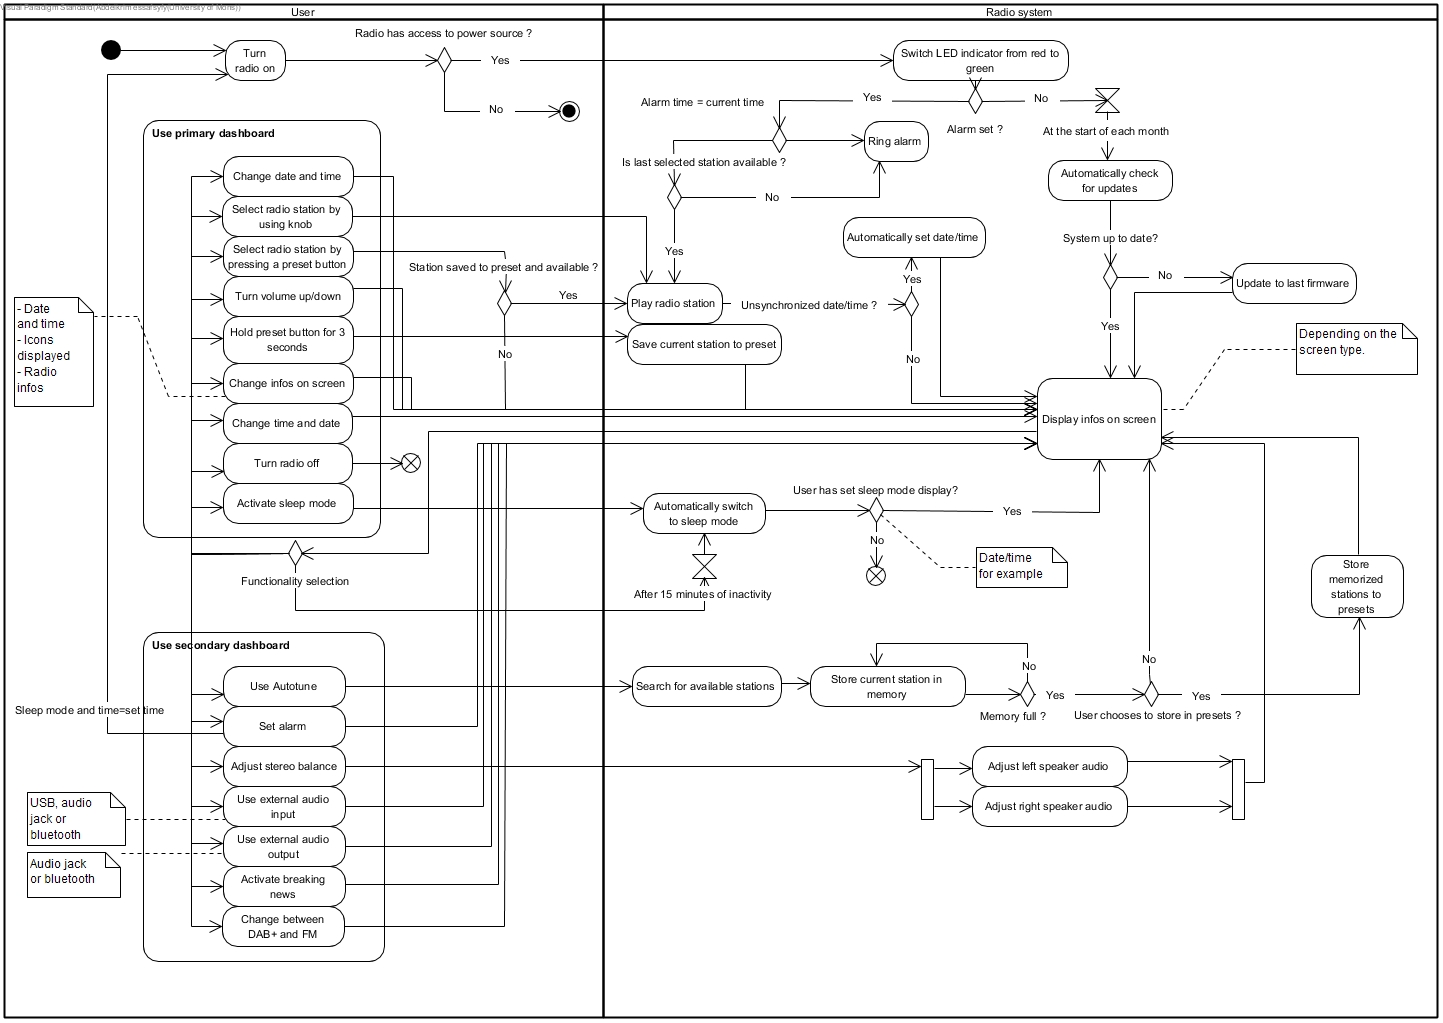
\includegraphics[width=15cm]{../Diagrams/Activity-v5.jpg}\\
\end{center}
While remaining consistent with the concept of two separate dashboards, we created the activity diagram following another -realistic- concept; the user can freely choose between functionalities, which means that the user can, for example, turn the volume up or down before choosing a station. In other words, most of the time, there are no mandatory sequences to follow.\\
In order the achieve this, we use a "hub" activity that will allow the user to switch from one action to the other. This "hub" activity is  "Display infos on screen", which makes sens since the user has to constantly receive feedback following their interaction with the radio. Doing so, we are able to start from any of the two dashboards and move on to whatever other action the user desires to do.\\
In order the make the diagram as legible as possible, some arrows (Control flows) are overlapping in a manner that avoids confusion as much as possible. Take secondary dashboard for example, it is clear that every functionality, except "Adjust stereo balance", once over, is redirected to the "hub" activity.\\
Finally, if the user has been inactive for 15 minutes, the radio automatically switches to sleep mode.

\pagebreak
\section{Interaction Overview diagram}
\vspace{10px}
\begin{center}
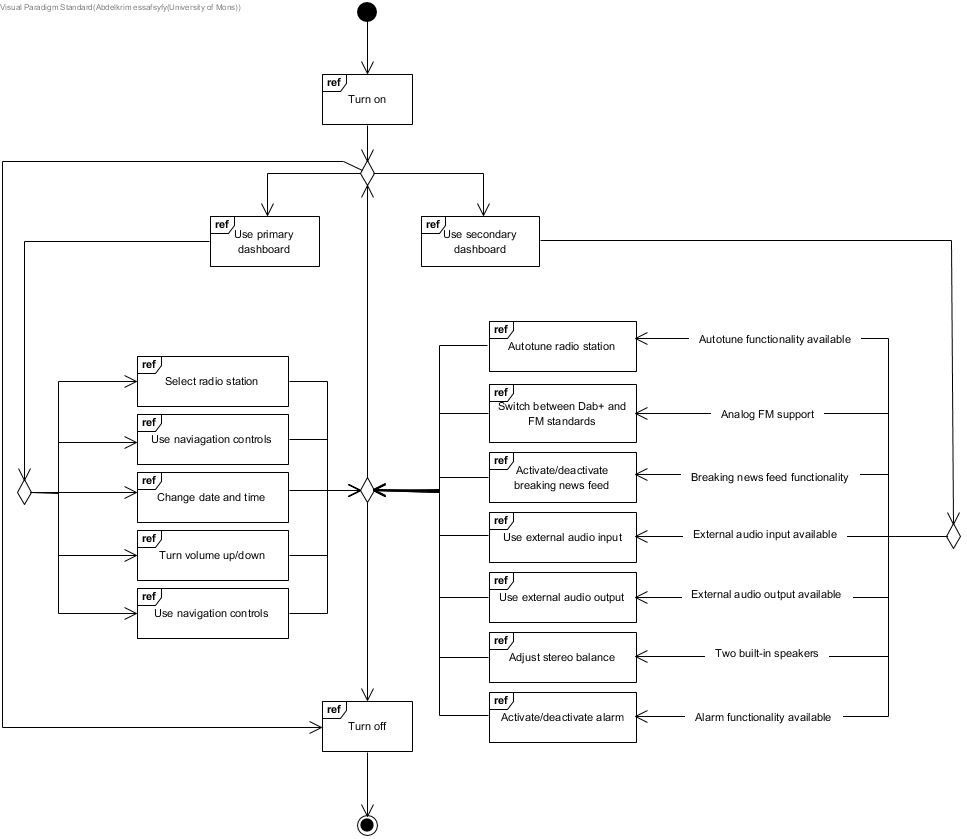
\includegraphics[width=15cm]{../Diagrams/InteractionOverview-v2.jpg}\\
\end{center}
In this interaction overview diagram, we specify the steps taken by the user when manipulating the radio. Please note that there aren't as many sequence diagrams as referenced in each interaction. If done so, most of the sequence diagrams would have been uninterestingly similar and repetitive.\\
The steps taken by the user are as follows:
\begin{enumerate}
\item The user turn the radio on
\item They choose to use either the primary or secondary dashboard (or turn the radio off)
\item Which leads them to choose on of the available functionalities in each category
\item Once the action is performed, the user can once again choose between the two categories
\item The user can also turn the radio off
\end{enumerate}

\pagebreak
\topskip0pt
\vspace*{\fill}
\begin{center}
Please note that every diagram present in this report will be available for viewing in the "Diagrams" folder.\\\vspace{30px}
If need be, a link to the \textit{Git} repository used for this project:\\
\url{https://github.com/Virtuosek/Radio}\\
Since the repository is private, you might get a 404 error if you're not a collaborator, if you wish to be one, please send an email to \href{mailto:karim.essaf@gmail.com}{karim.essaf@gmail.com} with your \textit{Git} username in order to be added as a collaborator\footnote{Be aware that we are only able to use the basic version of \textit{Git}, so only one collaborator can be added.}.
\end{center}
\vspace*{\fill}

\end{document}